% !TeX spellcheck = it_IT

\section{La ripartizione del Dominio}\label{sec:fourth_sudd_dom}
Come detto nel paragrafo \ref{subsec:partitioning}, la suddivisione del dominio (che avviene essenzialmente tramite \textit{graph-partitioning}) è un processo di pre-computazione fondamentale per la maggior parte delle applicazioni che lavorano su architetture distribuite. Infatti, un partizionamento corretto permette di sfruttare al meglio la potenza di calcolo offerta da un sistema di \textit{supercomputing}.\\
Vista la necessità di portare il progetto \textit{Shallow Water Equation on GPU} su un'architettura di nodi distribuita, così da poter raggiungere la potenza di calcolo richiesta per eseguire simulazioni in tempi ragionevoli, si è iniziato a modellare l'applicativo per poterlo adattare alla suddetta architettura.\\
In particolare questa tesi studia la ripartizione del dominio sui vari nodi.\\
In questo capitolo verrà quindi introdotto il \textit{criterio di suddivisione} studiato spiegando nel dettaglio la sua implementazione.\\
La suddivisione verrà affrontata in varie versioni che varieranno i risultati della ripartizione stessa dal punto di vista del bilanciamento (numero di elementi contenuti nei vari sotto-domini) e delle comunicazioni tra i vari sotto-domini.\\
Si procederà infine a fornire un confronto tra le varie versioni della suddivisione.

\subsection{La conformazione del dominio}
Prima di descrivere le varie operazioni di ripartizione è necessario però analizzare nel dettaglio il dominio stesso.\\
Come detto nel capitolo \ref{sec:first_swe}, il dominio reale del programma per la simulazione numerica dei flussi d’acqua, è una regione di territorio e tutte le informazioni che lo descrivono, vengono mappate nel dominio logico grazie alle celle e ai blocchi.\\
Ai fini della tesi verranno considerati solo i blocchi, senza tenere conto delle celle che li compongono, in quanto, le informazioni interessanti per la simulazioni vengono fornite dai blocchi stessi e non dalle singole celle che possono pertanto essere tralasciate.\\
In quest'ottica quando si parla di multi risoluzione ci si riferisce alla differenza di risoluzione dei blocchi e non delle celle che li compongono.\\

\subsubsection{Le caratteristiche del grafo}
Per rappresentare la conformazione del dominio reale all'interno del programma si è utilizzato un grafo diretto (paragrafo \ref{subsubsec:graph_type}) in cui l'insieme \textit{V} dei nodi è uguale all'insieme dei blocchi e l'insieme \textit{E} degli archi è composto dalle comunicazioni che ogni blocco ha con i relativi vicini.\\
La particolare conformazione di questo grafo fa sì che ogni blocco abbia un arco uscente e uno entrante per ogni vicino. Vista questa proprietà si assumerà d'ora in poi che il grafo sia indiretto e che l'adiacenza di un blocco con i vicini sia rappresentata da un solo arco $(blocco,vicino) \equiv (vicino,blocco)$ che sostituirà i due archi, quello entrante e quello uscente, senza alterare la struttura del dominio come si può vedere dalla figura \ref{fig:domain_graph}.\\
\begin{figure}[H]
	\centering
	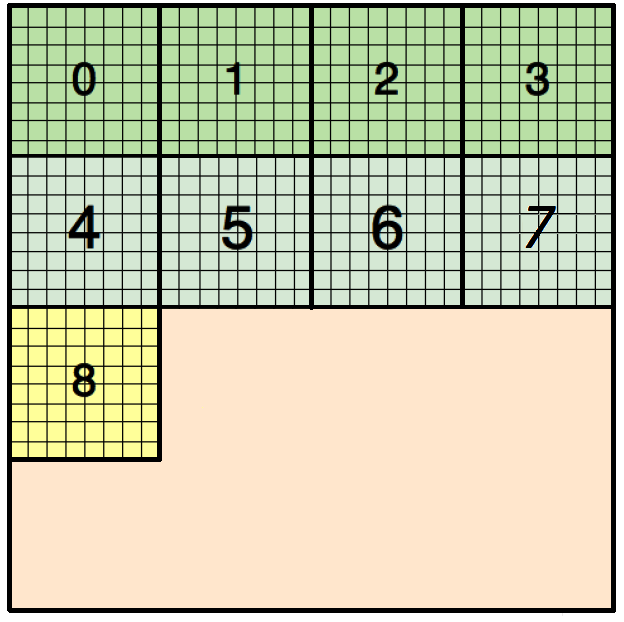
\includegraphics[width=1.0\textwidth]{immagini/block_on_grid.png}
	\caption{Grafo di un dominio reale senza multi risoluzione}
	\label{fig:domain_graph}
\end{figure}

\subsubsection{La rappresentazione del grafo}
La rappresentazione effettiva del grafo su macchina avviene attraverso l'array \textit{neigh} (paragrafo \ref{subsubsec:data_types_swe}) che combina i vantaggi di una rappresentazione a lista e matrice di adiacenza (paragrafo \ref{subsec:graph_rappr}). Questa combinazione è possibile grazie al numero piccolo (otto) di vicini di ogni blocco fissato a priori. Questa proprietà permette all'array \textit{neigh} di poter accedere efficientemente alle informazioni dei vicini di ogni blocco mantenendo comunque un'occupazione di memoria pari a $\Theta(V+E)$.\\
Ad esempio dato un blocco \textbf{K} è possibile controllare le informazioni di tutti i suoi vicini scorrendo le otto celle da \textit{neigh}[\textbf{K}$.id*8$] a \textit{neigh}[\textbf{K}$.id*8 + 7$]. Inoltre se si vuole controllare lo stato di un vicino in una determinata posizione (Nord, Sud, $\ldots$) basterà seguire lo schema indicato in figura \ref{fig:disp_neigh} al capitolo \ref{sec:first_swe} ed utilizzare l'indice relativo alla posizione voluta: le informazioni sul vicino Nord di \textbf{K}, ad esempio, si possono ricavare, con un singolo accesso, nella cella \textit{neigh}[\textbf{K}.$id*8 + 6$], essendo il vicino Nord associato all'indice 6.

\subsubsection{La multi risoluzione nel grafo}
La topologia del grafo che rappresenta il dominio è profondamente influenzata dal concetto di multi risoluzione la cui presenza varia significativamente il rapporto tra la quantità di nodi presenti e l'ampiezza del terreno tra le zone di alto e basso interesse. Un'alta risoluzione crea quindi zone computazionalmente pesanti e nelle quali intercorrono grandi quantità di connessioni mentre, al contrario, zone a basse risoluzioni sono contraddistinte da un esiguo numero di blocchi e da poche comunicazioni.\\
Questa differenza tra le zone a diverse risoluzioni sarà il punto centrale dell'algoritmo di partizionamento. Questo infatti, cercherà di suddividere il dominio in modo che le zone ad alto costo computazionale siano distribuite equamente tra i vari sotto-domini eseguendo il \textit{taglio} in zone con un basso numero di comunicazioni al fine di ridurre l'\textit{overhead} dovuto allo scambio dei dati.
\begin{figure}[H]
	\centering
	\begin{subfigure}{1.0\textwidth}
		\centering
		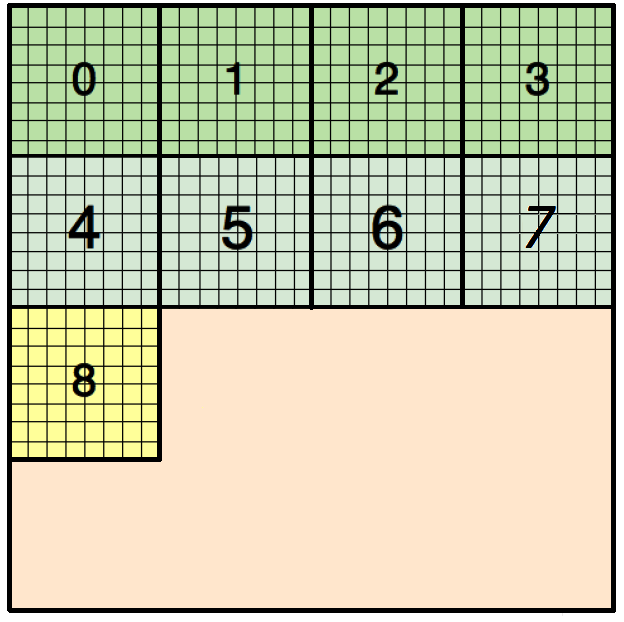
\includegraphics[width=1.0\linewidth]{immagini/block_on_grid.png}
		\caption{Grafo con vertici proporzionali alla zona di terreno rappresentata\newline}
		\label{fig:graph_multi}
	\end{subfigure}
	\begin{subfigure}{1.0\textwidth}
		\centering
		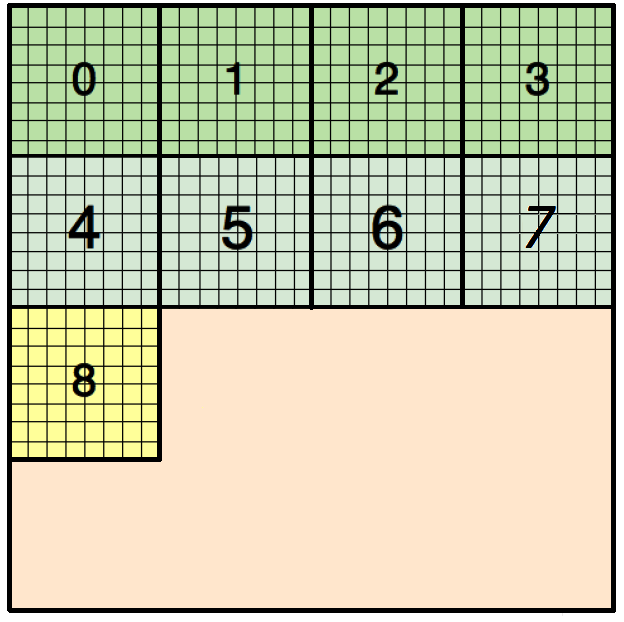
\includegraphics[width=1.0\linewidth]{immagini/block_on_grid.png}
		\caption{Grafo con vertici uniformi}
		\label{fig:graph_multi_equiv}
	\end{subfigure}
	\caption{Grafo di un dominio reale con multi risoluzione}
	\label{fig:domain_graph_multi}
\end{figure}

Il grafo d'ora in avanti sarà rappresentato con vertici rettangolari e senza rappresentare gli archi che connettono i vari nodi. Questa rappresentazione (realizzata tramite l'applicativo Graphviz \cite{graphviz}), mostrata in figura \ref{fig:square_graph} permette una migliore visione d'insieme del dominio
\begin{figure}[H]
	\centering
	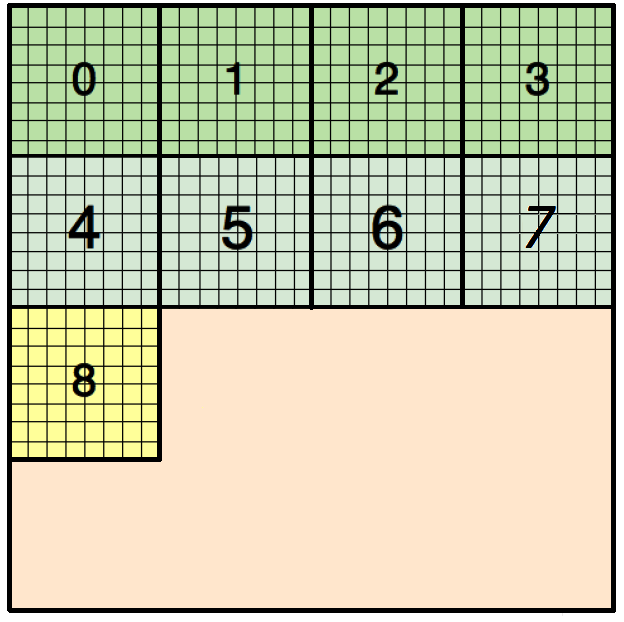
\includegraphics[width=1.0\linewidth]{immagini/block_on_grid.png}
	\caption{Modello di rappresentazione utilizzato}
	\label{fig:square_graph}
\end{figure}

\subsection{Le strutture dati dell'algoritmo}
Lo sviluppo dell'algoritmo ha richiesto l'introduzione di alcune strutture dati che permettessero di poter elaborare efficientemente il dominio, legando ad ogni nodo del grafo (ovvero ad ogni blocco) informazioni aggiuntive.\\
Si è quindi sviluppato il tipo di dato \emph{Block} (mostrato nel codice \ref{lst:block_struct}) che permette di salvare al suo interno, oltre alle informazioni fornite dal grafo di partenza (\textit{id\_block, id\_resolution, neighbors}), altri parametri utili all'algoritmo di suddivisione.\\
\begin{lstlisting}[ 
label={lst:block_struct},
caption={Struttura dati \textit{Block}}]
	struct Block
	{
		int id_block;
		char resolution;
		int id_subdomain;
		int key;
		bool in_other_subdomain;
		struct neigh_t neighbors[4];
	};
\end{lstlisting}
\textit{Block} cambia leggermente la modalità di memorizzazione dei vicini trasportandone tutte le informazioni nell'array \textit{neighbors} che mantiene comunque il tipo \textit{neigh\_t} (paragrafo \ref{subsubsec:data_types_swe}) per la memorizzazione dei vicini).\\
Al contrario di quello che ci si aspetterebbe la dimensione di \textit{neighbors} è quattro e non otto. Questo è dovuto al fatto che le comunicazioni del blocco con i vicini diagonali avvengono solo in casi di adiacenza particolari e quindi non influenzano i criteri per la suddivisione. L'associazione tra indice e posizione del blocco viene comunque mantenuta introducendo un nuovo schema mostrato in figura \ref{fig:new_scheme_neigh}.\\
\begin{figure}[H]
	\centering
	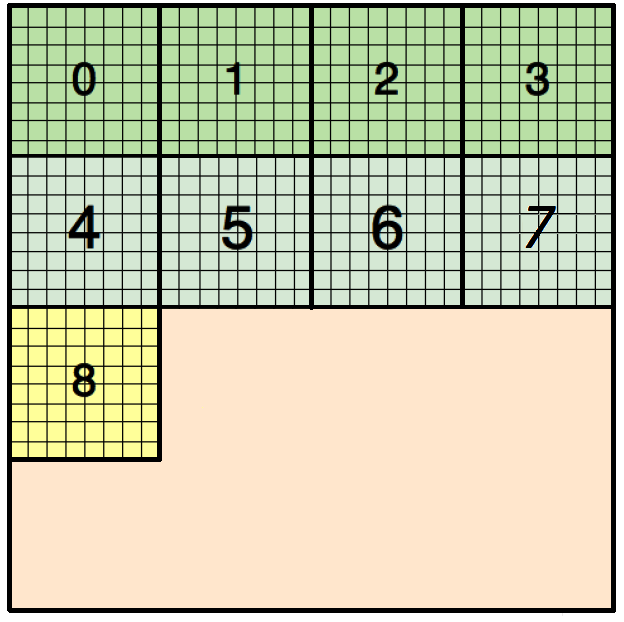
\includegraphics[width=1.0\textwidth]{immagini/block_on_grid.png}
	\caption{Il nuovo schema di associazione}
	\label{fig:new_scheme_neigh}
\end{figure}

Il grafo, durante il partizionamento, sarà rappresentato quindi da un array di \textit{Block}, chiamato \emph{adjacency\_list}, che rispecchia le proprietà di \textit{neigh}.

\subsection{La suddivisione tramite multi-MST}
Introdotte le strutture dati principali e spiegata la conformazione del grafo si possono passare a descrivere i primi stadi dell'algoritmo pensato per trovare una buona suddivisione.\\
Una buona ripartizione del dominio sui vari nodi di calcolo dovrebbe, come detto prima, soddisfare due requisiti:
\begin{itemize}
	\item Bilanciare la quantità di informazioni, e quindi il numero di blocchi, fra tutti i sotto-domini;
	\item Ridurre al minimo il numero di comunicazioni tra i nodi di calcolo cercando quindi di eseguire i \textit{tagli} al grafo in zone in cui intercorrono pochi \textit{archi}.
\end{itemize}

Considerando la multi risoluzione e la conseguente topologia del grafo i due parametri citati precedentemente possono essere rivisti nei seguenti termini:
\begin{itemize}
	\item Suddividere più equamente possibile le zone a risoluzione più alta;
	\item Eseguire i \textit{tagli} nelle zone a risoluzione più bassa.
\end{itemize}

L'idea su cui si basa l'algoritmo di partizionamento, che cerca di rispettare questi due requisiti, si fonda sul concetto di \textit{albero di copertura minimo} con archi equi-pesati (paragrafo \ref{subsec:mst_description}).\\
In particolare si utilizzerà una foresta di MST che esplorano il grafo contemporaneamente.\\


\subsubsection{Suddivisione di un dominio Ideale}
Inizialmente l'idea è nata immaginando di effettuare una suddivisione su un \emph{dominio ideale} in cui ci sono tante zone ad alta risoluzione quanti nodi di calcolo e dove queste degradano lentamente verso zone a risoluzione minima. Prendendo questo dominio è facile immaginarne una suddivisione ottimale tramite gli alberi di copertura minimi.\\
In particolare ogni albero di copertura minima, che rappresenta la partizione da assegnare ad un nodo di calcolo, ingloberebbe tutta una zona a risoluzione massima e i conseguenti contorni a risoluzioni intermedie, fermandosi (come mostrato nella figura \ref{fig:mst_stop}) quando incontra le \emph{foglie} di un altro MST (che avrà a sua volta inglobato nei suoi nodi interni le zone a risoluzione maggiore).\\
Data la configurazione ideale del dominio si può supporre che l'incontro fra i vari MST avvenga nelle zone di risoluzione minima individuando un'area nella quale è possibile  effettuare un \textit{taglio} che minimizza le comunicazioni.
\begin{figure}[H]
	\centering
	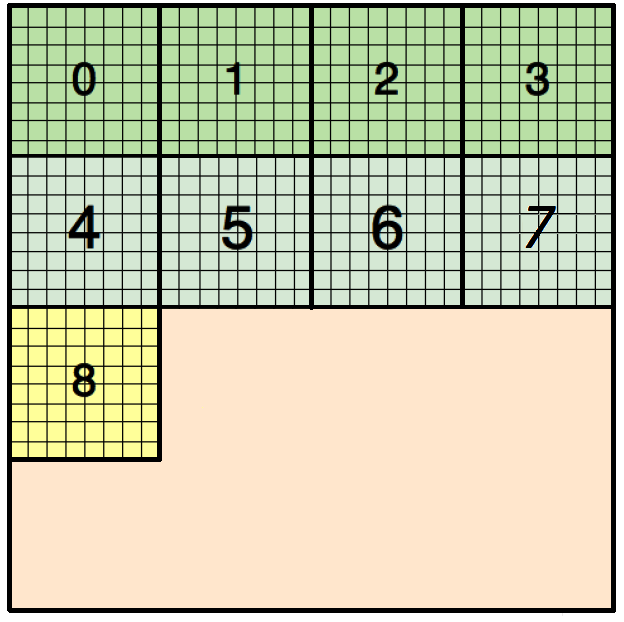
\includegraphics[width=0.5\textwidth]{immagini/block_on_grid.png}
	\caption{Le linee di arresto dei vari MST che compongono la foresta}
		\label{fig:mst_stop}
	\centering{In ogni vertice del grafo è mostrato il realtivo peso e il peso di ogni arco è considerato unitario}

\end{figure}
I problemi relativi a questo primo passo dell'algoritmo sono però evidenti: si richiede un dominio ideale e quindi non compatibile con i casi reali, gli unici che sono realmente interessanti, e inoltre si presuppone di conoscere a priori i blocchi di partenza che permettono all'algoritmo di eseguire una suddivisione ottimale.\\

\subsubsection{Le radici Casuali}\label{subsubsec:random_roots}
Il partizionamento tramite \emph{multi-MST} (ovvero l'esecuzione di più MST su uno stesso dominio) rimane però un buon punto di partenza. La suddivisione ottenuta grazie a questo approccio, se scelti buoni punti di partenza, riesce a sfruttare la topologia del grafo per creare partizioni bilanciate e \textit{tagli} con un basso numero di comunicazioni.\\
Partendo dalle giuste radici, i vari alberi di copertura minimi permetterebbero una divisione omogenea del numero dei blocchi.\\
Avendo infatti gli archi tutti lo stesso peso, la copertura di un albero si fermerà solo quando le foglie di questo incontreranno le foglie di un altro albero con un peso simile (come mostrato in figura \ref{fig:mst_stop}), indicando che il numero di blocchi inglobati è equilibrato.\\
Inoltre è possibile supporre che, se le radici fossero poste nei punti centrali delle zone a densità di informazione massimale\footnote{Con risoluzione più alta e con massima distanza dalle zone a risoluzione più bassa}, questo tipo di suddivisione permetterebbe di eseguire i \textit{tagli} nelle zone topologicamente più leggere e quindi dove intercorrono meno comunicazioni.\\
Idealmente infatti posizionando le radici nei punti \textquotedblleft più interni\textquotedblright (ovvero nei punti al centro delle zone più dense) del dominio, le zone sarebbero mappate sull'albero all'incirca in base alla loro concentrazione di blocchi. In particolare le zone a densità minore rappresenterebbero le foglie dell'albero e quindi le zone in cui viene eseguito il \textit{taglio}.\\
Come primo stadio dell'algoritmo su casi reali è stata realizzata una suddivisione basata su multi-MST che sceglie casualmente le proprie radici e che viene eseguita ripetutamente per poter scegliere una soluzione accettabile.\\
Nella (figura \ref{fig:random_root}) è mostrata una suddivisione con radici di partenza casuali.
\begin{figure}[H]
	\centering
	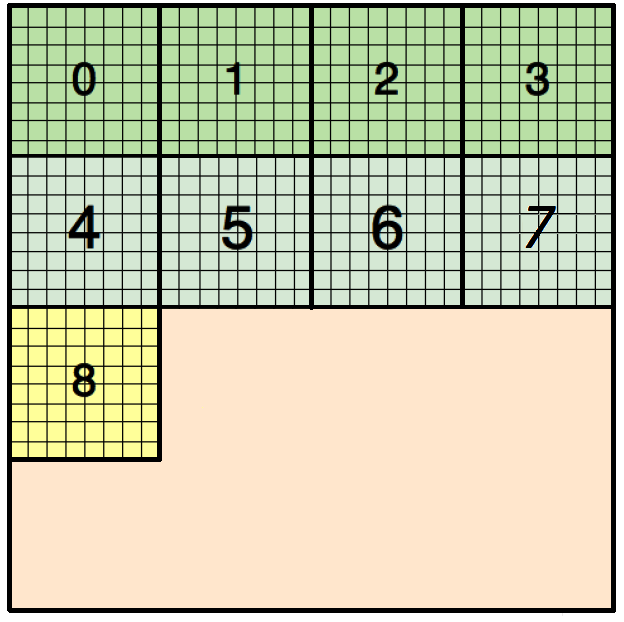
\includegraphics[width=0.9\textwidth]{immagini/block_on_grid.png}
	\caption{Ripartizione del dominio in quattro partendo da radici casuali}
		\label{fig:random_root}
\centering{Le radici sono messe in evidenza con colori diversi}

\end{figure}
\paragraph{L'implementazione dell'algoritmo di Prim con multi-radice}~\\
Nel codice \ref{alg:my_prim_multi} si dà una descrizione in pseudo-codice della versione dell'algoritmo di Prim (algoritmo {\ref{alg:Prim_Mst}), utilizzato per realizzare la suddivisione, che ammette un numero di \emph{radici}, e di conseguenza un numero di MST, parametrico.\\
\textit{roots} è la lista delle radici e \textit{adjacency\_list} rappresenta l'array di \textit{Block} citato precedentemente.
\begin{algorithm}[H]
	\caption{Prim Multi Source}
	\label{alg:my_prim_multi}
	\begin{algorithmic}[1]
		\Statex
		\Function{PRIM\_MULTI-MST}{roots\_list \textit{roots}, array\_Block \textit{adjacency\_list}}
		
		\State{\color{blue}{//Inizializzazione di tutti i vertici}}
		\For{ogni \textit{u} $\in$ \textit{adjacency\_list}}
		\Let{\textit{u.key}}{$\infty$}
		\Let{\textit{u.id\_subdomains}}{\textit{NIL}}
		\Let{\textit{u.in\_other\_subdomain}}{FALSE} 
		\EndFor
		
		\State{\color{blue}{//Inizializzazione di tutte le radici}}
		\Let{\textit{i}}{0}
		\For{ogni \textit{r} $\in$ \textit{roots}}
		\Let{\textit{r.key}}{0}
		\Let{\textit{r.id\_subdomains}}{\textit{i}}
		\Let{\textit{i}}{$i+1$}
		\EndFor
		\State{\textit{Q}: coda di priorita ordinata in base al campo 
			\textit{key}}
		\Let{\textit{Q}}{\textit{roots}}
		\Let{\textit{count}}{0}
		
		\While{count $<$ \textit{adjacency\_list.size}}
		\Let{\textit{u}}{EXTRACT-MIN(\textit{Q})}
		
		\If{!(\textit{u.in\_other\_subdomain})}
		\State{\color{blue}{//Essendo il minimo viene aggiunto definitivamente}}
		\Let{\textit{u.in\_other\_subdomain}}{TRUE}
		\State{\color{blue}{//Si analizzano i vicini}}
		\For{ogni \textit{v} $\in$ \textit{u.neighbors}}
		\State{\color{blue}{//In questo caso specifico il peso di ogni arco vale 1}}
		\If{$v \in adjacency\_list$ and ($u.key+1) < v.key$}
		\Let{\textit{v.key}}{$u.key+1$}
		\Let{\textit{v.subdomains}}{\textit{u.subdomains}}
		\Let{\textit{count}}{\textit{count} + 1}
		\EndIf
		\EndFor
		\EndIf
		\EndWhile
		\State \Return{}
		\EndFunction
	\end{algorithmic}
\end{algorithm}
Terminata l'esecuzione, per ricostruire i vari sotto-domini, basterà analizzare i campi \textit{id\_subdomain} di tutti gli elementi (blocchi) contenuti all'interno dell'array \textit{adjacency\_list}, oppure memorizzare, per esempio in un array di liste di interi, i vari \textit{id} relativi ai blocchi che compongono un determinato sotto-dominio ogni volta che un blocco viene inglobato definitivamente da un MST (algoritmo \ref{alg:my_prim_multi}, riga 19).

\subsection{La selezione delle radici}
Si è implementata una suddivisione basata sulle capacità degli alberi di copertura minimi di sfruttare la conformazione topologica del grafo con multi risoluzione, che utilizza però come radici vertici casuali, richiedendo così un alto numero di tentativi per ottenere una suddivisione soddisfacente.\\
Per ovviare al problema quindi, si è cercato un criterio di \emph{selezione delle radici}.\\
Il criterio che verrà proposto in questa tesi si baserà sul concetto di \emph{massimo locale}.\\
Prima di introdurre il concetto di massimo locale però è necessario parlare di \emph{distance transform}.

\subsubsection{Distance Transform e Massimi Locali}\label{subsubsec:local_max_map_transf}
Il concetto di \textit{distance transform} o \textit{distance map} è solitamente legato alla rappresentazione di immagini e consiste nel trasformare un'immagine binaria\footnote{con solo 2 livelli di colore, tipicamente il bianco e il nero} in un'immagine a scala di grigi \cite{distance_transform}. Questa trasformazione mantiene invariata la struttura dell'immagine ma \textquotedblleft sfuma\textquotedblright~il livello di colore partendo dai punti più interni ed arrivando, con i toni più chiari, ai bordi dell'immagine.
\begin{figure}[H]
	\centering
	\begin{subfigure}{0.5\textwidth}
	\centering
	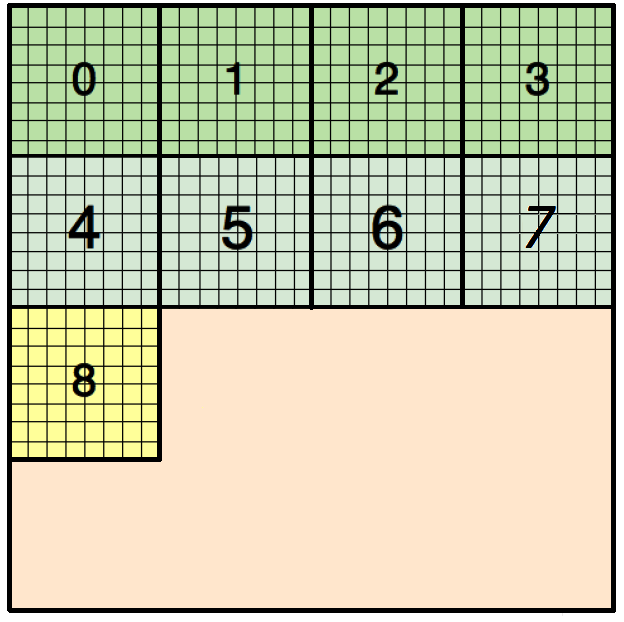
\includegraphics[width=0.5\textwidth]{immagini/block_on_grid.png}
	\caption{L'immagine prima della trasformazione}
	\end{subfigure}%
	\begin{subfigure}{0.5\textwidth}
	\centering
	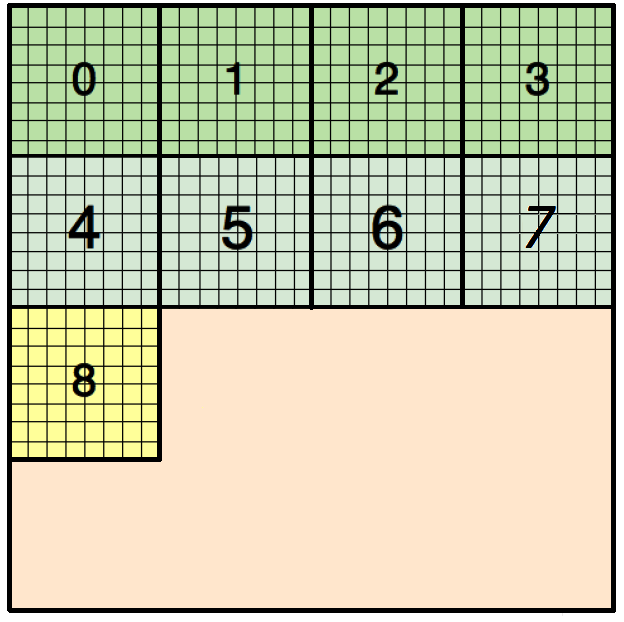
\includegraphics[width=0.5\textwidth]{immagini/block_on_grid.png}
	\caption{La stessa immagine dopo la trasformazione}
    \end{subfigure}
	\caption{Esempio di \textit{distance transform} su immagine binaria}
	\label{fig:map_transform_example}
\end{figure}

Lo stesso concetto può essere applicato al contrario, ovvero: dati i punti più esterni, si può \textquotedblleft sfumare\textquotedblright~verso quelli più interni cioè verso tutti quei punti con una massima distanza dai bordi rispetto ai loro vicini.\\
Una suddivisione di questo genere, applicata al dominio che si intende partizionare, permette di creare una distribuzione discreta e lineare di pesi.\\
In particolare si può utilizzare una specifica trasformazione \textit{distance map} che, partendo dai punti centrali delle zone a risoluzione minima locale (che comunicano cioè solo con zone a risoluzione maggiore), distribuisce i valori aumentandoli man mano che ci si allontana.\\
Dopo questa trasformazione si avrà quindi una \textquotedblleft curva\textquotedblright~della distribuzione delle risoluzioni ovvero, si passerà da una distribuzione di valori quantizzati\footnote{I valori rappresentano i vari livelli di risoluzione e sono: 1, 2, 3 e 4} molto distanti, ad una distribuzione più fitta. Questa distribuzione considera le distanze dalle risoluzioni vicine in modo da poter guidare una ricerca per gradiente dei massimi locali (figura \ref{fig:local_max_graph}).
I vertici del grafo che avranno associato un valore maggiore rispetto ai propri vicini, saranno identificati proprio come \emph{massimi locali} e rappresenteranno i punti più interni delle zone che hanno localmente la massima risoluzione.\\
\begin{figure}[H]
	\centering
	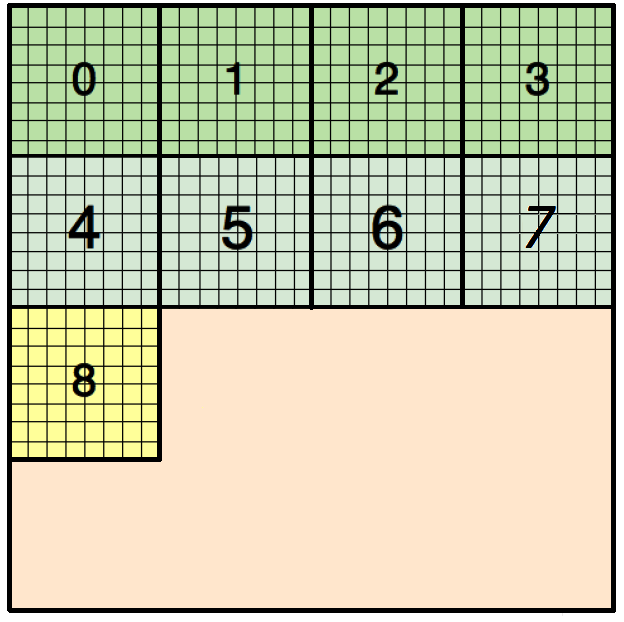
\includegraphics[width=1.0\textwidth]{immagini/block_on_grid.png}
	\caption{Grafo del dominio con i massimi locali evidenziati (in nero)}
	\label{fig:local_max_graph}
\end{figure}

Si illustra di seguito lo pseudo codice relativo alla trasformazione utilizzata sul dominio (che sfrutta l'algoritmo \ref{alg:my_prim_multi}) per l'individuazione dei massimi locali:
\begin{algorithm}[H]
	\caption{Map Tranform}
	\label{alg:my_map_transfor}
	\begin{algorithmic}[1]
		\Statex
		\Function{map\_tranform}{array\_Block \textit{adjacency\_list}}
		\State{\color{blue}{//Inizializzazione di tutti i vertici}}
		\For{ogni \textit{u} $\in$ \textit{adjacency\_list}}
		\Let{\textit{u.key}}{$\infty$}
		\Let{\textit{u.in\_other\_subdomain}}{FALSE} 
		\EndFor
		
		\State{\color{blue}{//Si analizza il grafo un livello di risoluzione alla volta}}		\Let{\textit{res}}{\textit{min\_res\_value}}
		\While{\textit{res} $\leq$ \textit{max\_res\_value}}
		\State{\color{blue}{Si definisce \textit{adjacency\_list}(\textit{res\_value}) l'insieme}}
		\State{\color{blue}{dei nodi a risoluzione \textit{res\_value}}}	
		\Let{\textit{Q}}{\textit{adjacency\_list}(\textit{res\_value})}
		\Let{is\_L}{FALSE}
		\While{{Q} $\neq 0$}
		\If{EXISTS\_LOW(\textit{Q})\color{orange}{$^1$}\color{black} and \textit{res} $\neq$ \textit{min\_res\_value}}
		\Let{\textit{start\_node}}{EXTRACT\_BOUNDARY\_L(\textit{Q})\color{orange}{$^2$}\color{black}}
		\Let{\textit{is\_L}}{TRUE}
		\Else
		\Let{\textit{start\_node}}{EXTRACT\_BOUNDARY\_H(\textit{Q})\color{orange}{$^3$}\color{black}}
		\EndIf
		\State{MST\_WEIGHT\_DIST(\textit{start\_node, is\_L, adjacency\_list, Q})\color{orange}{$^4$}}
		\EndWhile
		\EndWhile
		\State \Return{}
		\EndFunction
	\end{algorithmic}
\end{algorithm}
\begin{itemize}
\color{orange}\item[1]\color{black}EXISTS\_LOW (riga 10) verifica se è presente almeno un blocco che ha almeno un vicino a risoluzione minore;
\color{orange}\item[2]\color{black}EXTRACT\_BOUNDARY\_L (riga 11) estrae come blocco di partenza un blocco che comunica con vicini a risoluzione minore;
\color{orange}\item[3]\color{black}EXTRACT\_BOUNDARY\_H (riga 14) estrae un blocco che sia sul bordo del dominio o che abbia almeno un vicino a risoluzione maggiore;
\color{orange}\item[4]\color{black}MST\_WEIGHT\_DIST (riga 15) spiegato nell'algoritmo \ref{alg:dist_weight_mst}.
\end{itemize}

\begin{algorithm}[H]
	\caption{MST Weight Redistribution}
	\label{alg:dist_weight_mst}
	\begin{algorithmic}[1]
		\Statex
		\Function{MST\_WEIGHT\_DIST}{Block \textit{start\_node}, bool \textit{is\_L}, array\_Block \textit{adjacency\_list}, list\_same\_res\ \textit{Q}}
	    \Let{T}{EXTRACT\_COMMUNICANT(\textit{Q}, \textit{res\_start})\color{mygreen}{$^1$}\color{black}}
		
		\If{\textit{is\_L}}
	   
		\Let{\textit{list\_start\_node}}{COMPLETE\_BOUNDARY\_L(\textit{start\_node}, \textit{T})\color{mygreen}{$^2$}\color{black}}
		
		\Let{\textit{new\_start}}{PRIM\_MULTI-MST\_central(\textit{list\_start\_node}, \textit{T})\color{mygreen}{$^3$}\color{black}}
		\Let{\textit{T}[\textit{new\_start}]\textit{.key}}{0}
		\Else
		
	
		\Let{\textit{list\_start\_node}}{COMPLETE\_BOUNDARY\_H(\textit{start\_node}, \textit{T})\color{mygreen}{$^4$}\color{black}}
		\State{BOUNDARY\_WEIGHT(\textit{list\_start\_node}, \textit{adjacency\_list})\color{mygreen}{$^5$}\color{black}}
		\EndIf
		\State{PRIM\_MULTI-MST\_final(\textit{list\_start\_node}, \textit{T}, \textit{Q}, \textit{adjacency\_list})\color{mygreen}{$^6$}\color{black}}
		\State \Return{}
		\EndFunction
	\end{algorithmic}
\end{algorithm}
\begin{itemize}
\color{mygreen}\item[1]\color{black} EXTRACT\_COMMUNICANT (riga 2) estrae tutti i nodi di \textit{Q} che hanno comunicazione (diretta o indiretta) con \textit{start\_node} passando solo attraverso blocchi della stessa risoluzione;
\color{mygreen}\item[2]\color{black} COMPLETE\_BOUNDARY\_L (riga 4) estrae tutti i nodi nella zona di \textit{start\_node} (\textit{T}) che hanno stessa risoluzione e che possiedono almeno un vicino a risoluzione minore;
\color{mygreen}\item[3]\color{black} Si considera che la funzione PRIM\_MULTI-MST\_central (riga 5) esegua l'algoritmo \ref{alg:my_prim_multi} ma ritorni il nodo con valore \textit{key} maggiore senza modificare globalmente \textit{T};
\color{mygreen}\item[4]\color{black} COMPLETE\_BOUNDARY\_H (riga 8) estrae tutti i nodi nella zona di \textit{start\_node} (\textit{T}) che hanno stessa risoluzione e che possiedono almeno un vicino a risoluzione maggiore;
\color{mygreen}\item[5]\color{black}BOUNDARY\_WEIGHT (riga 9) ridefinisce i pesi delle radici (\textit{list\_start\_node}) assegnando ad ogni radice il peso del proprio vicino (anche a risoluzione minore) \textquotedblleft meno pesante\textquotedblright aumentato di 1 (tutti gli archi hanno infatti peso unitario);
\color{mygreen}\item[6]\color{black} PRIM\_MULTI-MST\_final (riga 10) esegue l'algoritmo \ref{alg:my_prim_multi} su \textit{T} senza settare a 0 il valore \textit{key} delle radici. Inoltre estrae da \textit{Q} tutti i blocchi in \textit{T} e riporta le modifiche sui valori dei blocchi in \textit{adjacency\_list}.
\end{itemize}


\subsubsection{I massimi locali randomici come partenza}
Grazie all'algoritmo \ref{alg:my_map_transfor} è quindi possibile determinare tutti i massimi locali del grafo; essendo questi i punti più interni del grafo, come detto nel paragrafo \ref{subsubsec:random_roots}, costituiscono delle buone radici per i vari MST.\\
Siccome il numero di partizioni desiderate è quasi sempre di molto inferiore al numero di massimi locali trovati, nasce il problema di quali scegliere come punti di partenza.\\
Un primo approccio è stato quello di scegliere le radici dell'algoritmo di partizione (algoritmo \ref{alg:my_prim_multi}) casualmente tra tutti i massimi locali (figura \ref{fig:randomo_local_max}).\\
Come si nota in figura \ref{fig:randomo_local_max} però questo approccio non garantisce affatto una suddivisione ideale.
\begin{figure}[H]
	\centering
	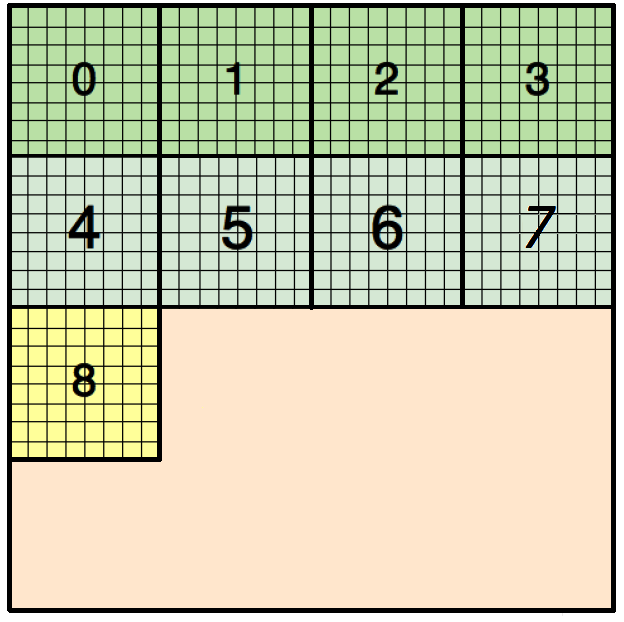
\includegraphics[width=1.0\textwidth]{immagini/block_on_grid.png}
	\caption{Ripartizione del dominio in quattro partendo da radici scelte casualmente tra i massimi locali}
	\label{fig:randomo_local_max}
\end{figure}


\subsection{Multi-MST sui massimi locali}
Calcolati tutti i massimi locali bisogna quindi cercare di sfruttarli per produrre una buona suddivisione.\\
I massimi locali sono, come definito nel paragrafo \ref{subsubsec:local_max_map_transf}, i punti centrali delle zone a densità di informazione massimale (risoluzione più alta e lontana da zone a risoluzione più bassa) e quindi delle zone più dense del grafo. Vista la posizione dei massimi locali è facile immaginare che nelle loro vicinanze vi sia un'alta concentrazione di blocchi e, di conseguenza un alto numero di comunicazioni.\\
Se si prende, per esempio, il dominio in figura \ref{fig:local_max_graph} nel quale sono stati calcolati i massimi locali risulta infatti evidente che le zone dove intercorrono meno comunicazioni sono quelle più distanti dai vari massimi locali.\\
Questo è dovuto proprio al fatto che i massimi locali sono al centro delle zone più pesanti dal grafo e quindi allontanandosi da questi si arriva su zone con una bassa densità di blocchi (zone a bassa risoluzione).\\

\subsubsection{Zone di appartenenza e Tagli ideali}\label{subsubsec:zone_app}
Vista questa proprietà si può quindi supporre che sia conveniente effettuare i \textit{tagli} tra i blocchi topologicamente più distanti dai vari massimi locali.\\
Per individuare queste zone si è sfruttata ancora una volta l'idea di albero di copertura minimo.\\
In particolare si è pensato di sviluppare contemporaneamente, sullo stesso dominio, un MST per ogni massimo locale (con radice nel massimo locale stesso) utilizzano l'algoritmo \ref{alg:my_prim_multi}.\\
Quando l'algoritmo ha terminato la sue esecuzione si potranno distinguere nel grafo le varie \textquotedblleft \emph{zone di appartenenza}\textquotedblright, una per ogni massimo locale (figura \ref{fig:mst_local_max}).
\begin{figure}[H]
	\centering
	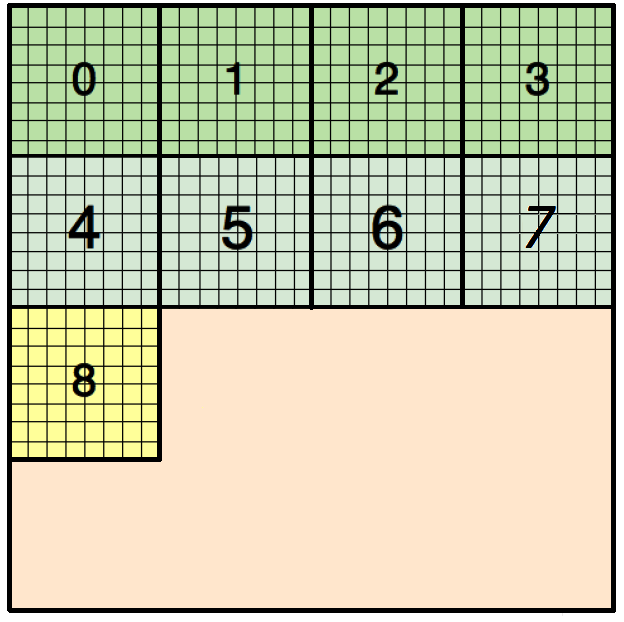
\includegraphics[width=1.0\textwidth]{immagini/block_on_grid.png}
	\caption{Le zone di appartenenza descritte dalla foresta di MST}
	\label{fig:mst_local_max}
\end{figure}

Una volta definite le \textquotedblleft zone di appartenenza\textquotedblright~risulta quindi chiaro che i bordi esterni dei vari MST rappresentano le zone più distanti dai massimi locali.\\
In particolare, seguendo l'idea che nelle nelle zone più lontane dai massimi locali ci sia minima comunicazione, i vari \textit{tagli} dovrebbero essere effettuati lungo \emph{le linee di contatto} (mostrate in figura \ref{fig:mst_stop}) tra i vari MST.\\
Tagliando lungo le suddette linee infatti è possibile evitare di \textit{tagliare} dove vi è una grande densità di blocchi.\\
Si può dire quindi che le \textit{linee di contatto} forniscano le zone ideali su cui effettuare i vari \textit{tagli} necessari a partizionare il grafo.

\subsubsection{Unione delle zone di appartenenza}\label{subsubsec:varius_merge}
Definite le linee lungo le quali effettuare i possibili \textit{tagli} è il momento di suddividere il grafo vero e proprio nel numero di partizioni desiderato.\\
Per mantenere intatte le zone di taglio sicure si è pensato di eseguire la suddivisione partendo proprio dalle \textit{zone di appartenenza}.\\
Unendo tra loro le singole zone è possibile infatti creare sotto-domini maggiori che conservino le \textit{linee di taglio} individuate precedentemente e che producano quindi un buon partizionamento del grafo.\\
Perciò si è usato un processo di unione iterativo che ad ogni passo seleziona i due sotto-domini migliori da unire fino a raggiunger il numero di partizioni volute.\\
Siccome vi sono diversi criteri di unione validi, questo algoritmo di unione è stato sviluppato in più versioni ognuna delle quali può variare sia nella scelta iniziale del sotto-dominio che si vuole unire, sia nella scelta della partizione da unire con il suddetto sotto-dominio.\\
In particolare si avranno i seguenti criteri:
\begin{itemize}
	\item[1] Si sceglie come sotto-dominio di partenza quello con il rapporto\\
	$numero\_blocchi\mathbin{/}numero\_comunicazioni$ peggiore (cioè minore) e come partizione da unire quella che riduce maggiormente le comunicazioni del sotto-dominio di partenza (figura \ref{fig:nb_comm});
	\item[2] Si sceglie come sotto-dominio di partenza quello con il rapporto\\
	$numero\_blocchi\mathbin{/}numero\_comunicazioni$ peggiore (cioè minore) e come partizione da unire quella che, unita al sotto-dominio di partenza, produce il rapporto $numero\_blocchi\mathbin{/}numero\_comunicazioni$ migliore (figura \ref{fig:nb_nb});
	\item[3] Si sceglie come sotto-dominio di partenza quello con il più alto numero di comunicazioni e come partizione da unire quella che,che riduce maggiormente le comunicazioni del sotto-dominio di partenza (figura \ref{fig:comm_comm}).
\end{itemize}
Tutti e tre i vari criteri sono suddivisi in altre due versioni: una che ammette la possibilità di eseguire un'unione anche tra vicini non adiacenti per permettere un bilanciamento migliore, e un'altra che non lo consente (a meno di un grande sbilanciamento nei sotto-domini finali).\\
\begin{figure}[H]
	\centering
	\begin{subfigure}{1.0\textwidth}
	\centering
		\begin{subfigure}{0.5\textwidth}
			\centering
			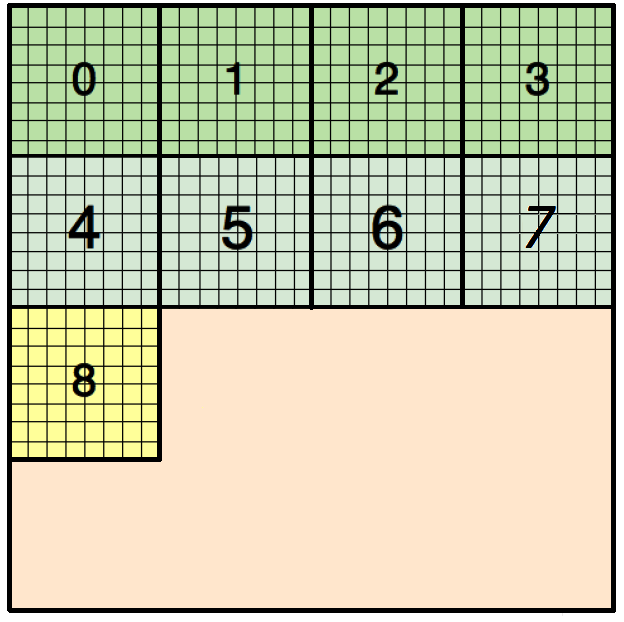
\includegraphics[width=0.9\textwidth]{immagini/block_on_grid.png}
			Amessi solo vicini adiacenti
		\end{subfigure}%
		\begin{subfigure}{0.5\textwidth}
			\centering
			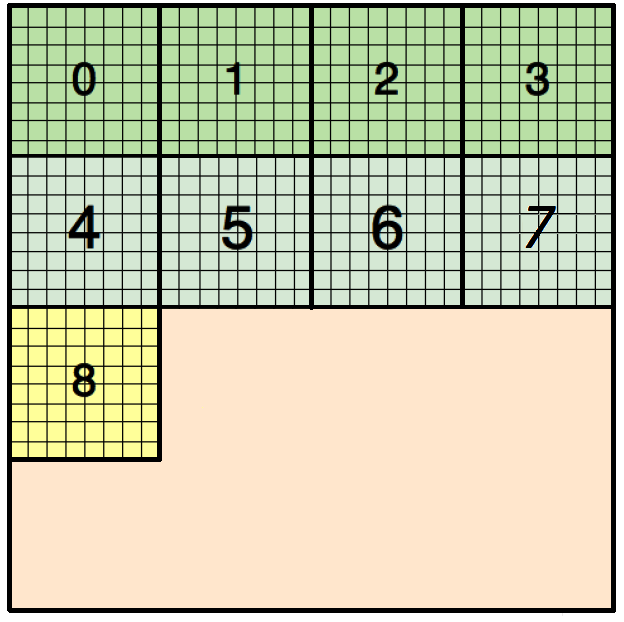
\includegraphics[width=0.9\textwidth]{immagini/block_on_grid.png}
			Vicini non adiacenti ammessi
		\end{subfigure}
	\caption{Ottimizzazione rapporto $numero\_blocchi\mathbin{/}numero\_comunicazioni$ e comunicazioni\newline}
	\label{fig:nb_comm}
	\end{subfigure}
	\begin{subfigure}{1.0\textwidth}
	\centering
		\begin{subfigure}{0.5\textwidth}
			\centering
			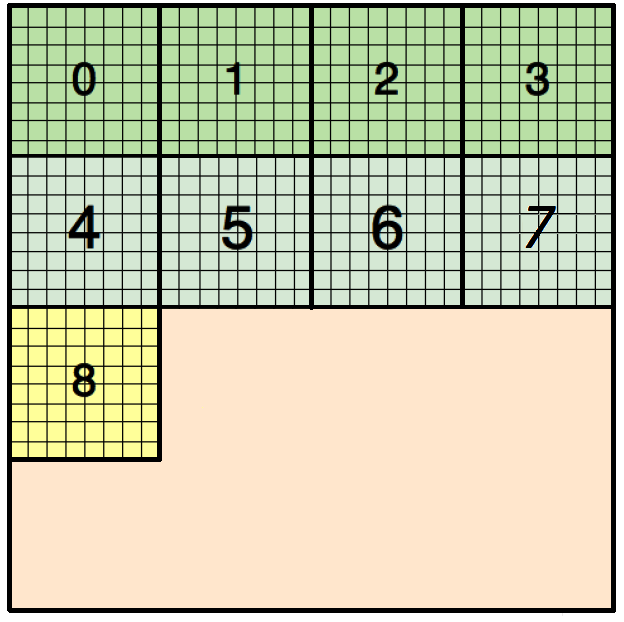
\includegraphics[width=0.9\textwidth]{immagini/block_on_grid.png}
			Amessi solo vicini adiacenti
		\end{subfigure}%
		\begin{subfigure}{0.5\textwidth}
			\centering
			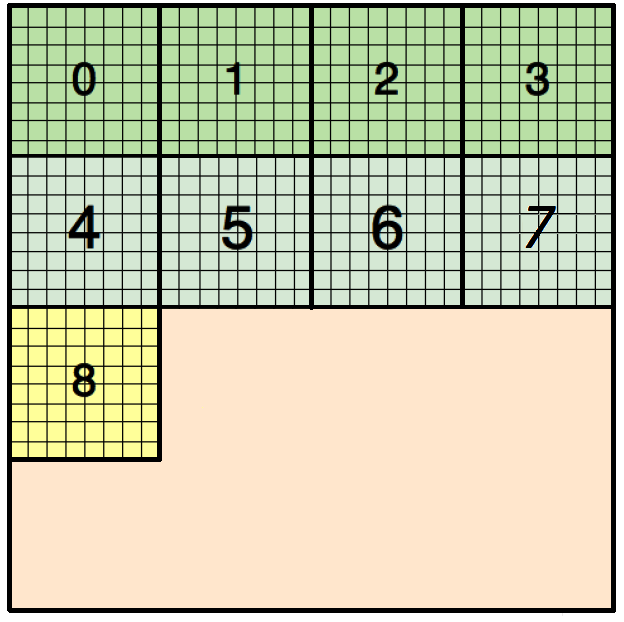
\includegraphics[width=0.9\textwidth]{immagini/block_on_grid.png}
			Vicini non adiacenti ammessi
		\end{subfigure}
	\caption{Ottimizzazione rapporto $numero\_blocchi\mathbin{/}numero\_comunicazioni$\newline}
	\label{fig:nb_nb}
	\end{subfigure}
	\begin{subfigure}{1.0\textwidth}
	\centering
	\begin{subfigure}{0.5\textwidth}
		\centering
		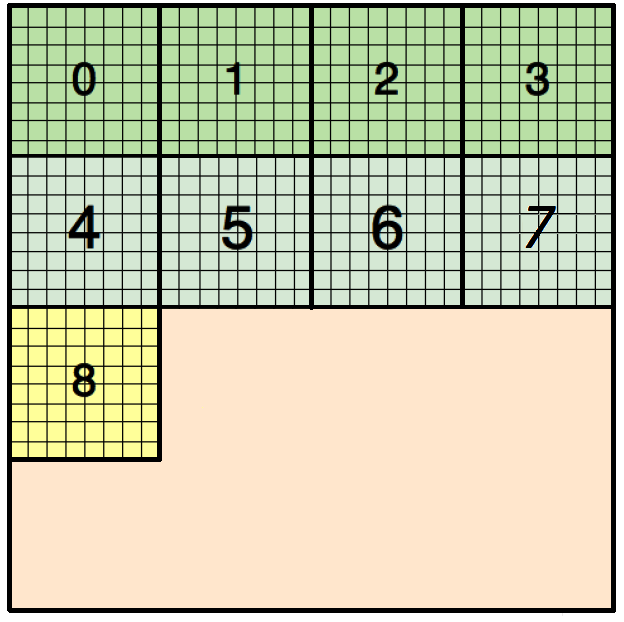
\includegraphics[width=0.9\textwidth]{immagini/block_on_grid.png}
		Amessi solo vicini adiacenti
	\end{subfigure}%
	\begin{subfigure}{0.5\textwidth}
		\centering
		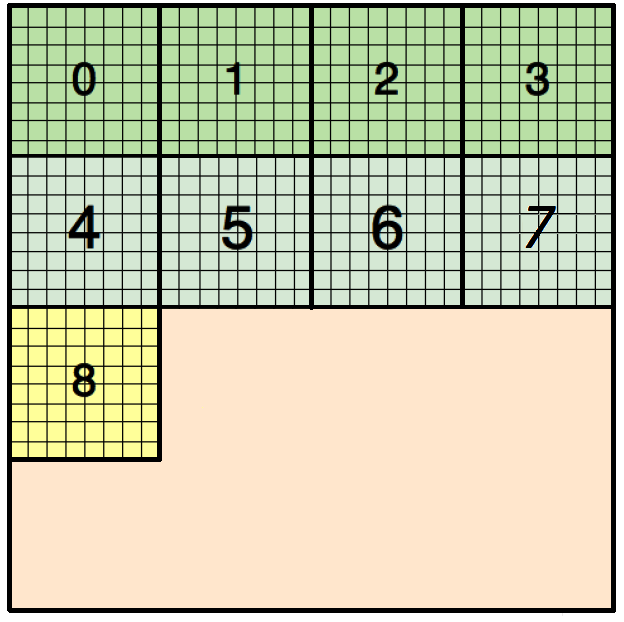
\includegraphics[width=0.9\textwidth]{immagini/block_on_grid.png}
		Vicini non adiacenti ammessi
	\end{subfigure}
	\caption{Ottimizzazione comunicazioni\newline}
	\label{fig:comm_comm}
\end{subfigure}
	\caption{I vari criteri di unione a confronto}
\end{figure}

I vari criteri di unione creano diverse suddivisioni all'interno dello stesso grafo ma producono comunque delle ripartizioni accettabili, sia dal punto di vista del bilanciamento che dal punto di vista dell comunicazioni, senza richiedere diversi tentativi come invece accade nelle implementazioni basate su radici casuali.\\
Si è quindi riusciti ad ottenere una suddivisione soddisfacente del dominio, che permette di ripartire il carico adeguatamente su una struttura MPI.


\subsection{I confronti}
Nell'immagine \ref{fig:comm_confronto} si mostreranno due grafici che valutano in base a due parametri (il bilanciamento e il numero delle comunicazioni totali) le varie fasi dell'algoritmo e i vari criteri di unione delle \textit{zone di appartenenza} (paragrafo \ref{subsubsec:varius_merge}).\\
In particolare si sono messi a confronto i vari criteri di unione, tra loro e con altri algoritmi di suddivisione basati sulla posizione dei blocchi o su scelte di radici casuali.
%\begin{itemize}
%	\item [1] Prim multi-MST con unione che ottimizza il numero delle comunicazioni;
%	\item [2] Prim multi-MST con unione che ottimizza il numero delle comunicazioni consentendo anche unione tra sotto-domini non adiacenti;
%	\item [3] Prim multi-MST con unione che ottimizza il rapporto $numero\_blocchi\mathbin{/}numero\_comunicazioni$ e il numero di comunicazioni;
%	\item [4] Prim multi-MST con unione che ottimizza il rapporto $numero\_blocchi\mathbin{/}numero\_comunicazioni$ e il numero di comunicazioni consentendo anche unione tra sotto-domini non adiacenti;
%	\item [5] Prim multi-MST con unione che ottimizza il rapporto $numero\_blocchi\mathbin{/}numero\_comunicazioni$;
%	\item [6] Prim multi-MST con unione che ottimizza il rapporto $numero\_blocchi\mathbin{/}numero\_comunicazioni$ consentendo anche unione tra sotto-domini non adiacenti;
%	\item [7] Suddivisione del dominio suddividendo in parti uguali l'asse \textit{x};
%	\item [8] Suddivisione del dominio suddividendo in parti uguali l'asse \textit{y};
%	\item [9] Suddivisione tramite multi-MST che utilizza come punti di partenza posizioni casuali (risultato migliore su 50 tentativi);
%	\item [10] Suddivisione tramite multi-MST che utilizza come punti di partenza \textit{massimi locali} casuali (risultato migliore su 50 tentativi);	
%\end{itemize}
\begin{figure}[H]
	\centering
	\begin{subfigure}{1.0\textwidth}
		\centering
		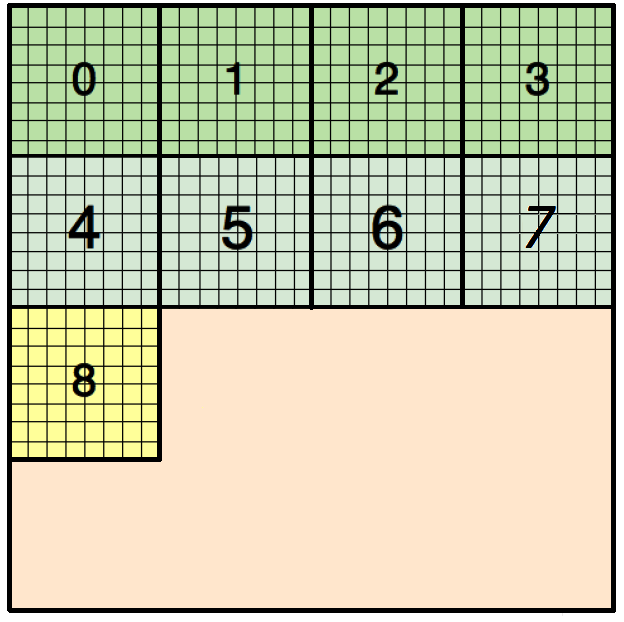
\includegraphics[width=0.9\textwidth]{immagini/block_on_grid.png}
		\caption{Il confronto degli algoritmi con quattro partizioni\newline}
		\label{fig:confronto_4}
	\end{subfigure}
	\begin{subfigure}{1.0\textwidth}
		\centering
		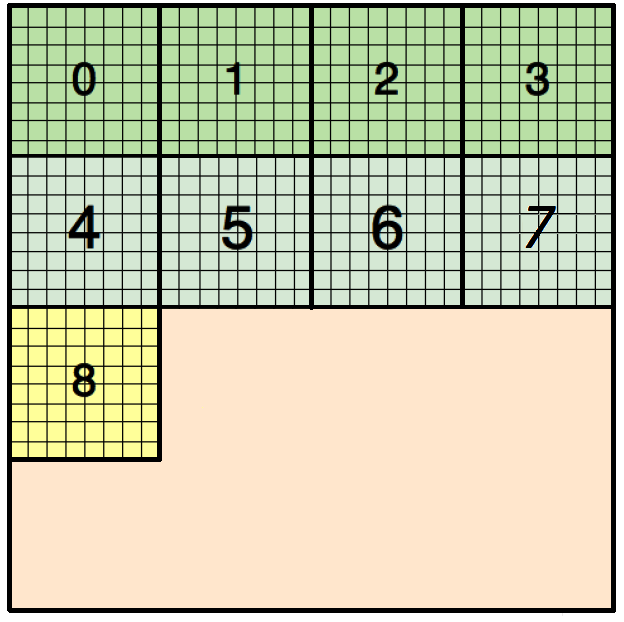
\includegraphics[width=0.9\textwidth]{immagini/block_on_grid.png}
		\caption{Il confronto degli algoritmi con otto partizioni}
		\label{fig:confronto_8}
	\end{subfigure}

	\caption{Le varie suddivisioni a confronto}
		\label{fig:comm_confronto}
\end{figure}


Nei grafici in figura \ref{fig:comm_confronto} non emerge, come ci si aspetterebbe, un miglioramento sul numero delle comunicazioni tra le suddivisioni basate sulle zone di appartenenza rispetto a quelle in cui si sono scelte radici casuali. Si nota anzi, che la suddivisione basata sull'offset ottimizza il numero di comunicazioni: questo è probabilmente dovuto alla conformazione del dominio e non è attribuibile ad una vera e proprio caratteristica della suddivisione.\\
Per quanto riguarda il bilanciamento invece, le suddivisioni basate sulle zone di appartenenza, ottengono dei buoni risultati rispetto alle altre. In particolare, si ottengono dei buoni risultati quando si ammettono anche unioni tra sotto-domini non adiacenti.

\subsubsection{Il risultato finale}
Il risultato dei confronti tra i vari algoritmi di ripartizione (figura \ref{fig:comm_confronto}), non fa emergere, come ci si aspetterebbe, un netto miglioramento sul numero di comunicazioni dovuto alla tecnica di suddivisione basata sulle \textit{zone di appartenenza}.\\
Questo è dovuto al fatto che il criterio di ripartizione basato sulle \textit{zone di appartenenza}, suddivide il dominio basando la sua esecuzione su zone che non cambiano mai la loro forma di base; infatti ogni sotto-dominio finale è semplicemente l'unione dei diversi MST iniziali.\\
Lo scarso miglioramento, rispetto ad algoritmi che si basano su scelte casuali, è quindi probabilmente dovuto alla struttura non ideale del \textit{taglio}, dettata dalla rigidità dei sotto-domini di base. Si può concludere che l'algoritmo basato sulle \textit{zone di appartenenza}, riesca ad individuare dove sia più corretto eseguire i \textit{tagli}, ma non li esegua nel modo più adeguato.\\

Al contrario, l'ultima suddivisione proposta in questa tesi, garantisce sempre un buon bilanciamento dei blocchi tra le varie ripartizioni.\\
Questa proprietà è molto importante in quanto, anche se non se ne ha la certezza, la distribuzione non equilibrata del carico porterebbe ad un overhead molto alto. Infatti, anche se non è ancora stata sviluppata una versione che permetta di testare realmente le suddivisioni, sembra che lo squilibrio del carico sui vari nodi causi un maggiore rallentamento rispetto a quello dovuto ad un alto numero di comunicazioni.\\

L'algoritmo studiato, nella sua ultima versione (paragrafo \ref{subsubsec:zone_app}), ha l'interessante proprietà di individuare un partizionamento con un numero di comunicazioni accettabile e di garantire un bilanciamento quasi perfetto\footnote{Il bilanciamento è migliore se si permette di unire tra loro sotto-domini non adiacenti}.\\
L'idea di ripartizione proposta in questa tesi potrebbe essere quindi, con qualche piccolo aggiustamento, una buona base per produrre una suddivisione ottima su tutti i vari domini che l'applicativo \textit{sweGPU} deve elaborare, indipendentemente dalla loro confermazione specifica.\\
In particolare l'idea di partizionamento basata sull'esecuzione di una foresta di MST (con radici adeguate) su uno stesso dominio con multi risoluzione, sembra garantire una suddivisione migliore di quelle che verrebbero individuate con gli algoritmi di partizionamento classici\cite{krapis_lab}.
In particolare l'algoritmo che ottimizza il rapporto $numero\_blocchi\mathbin{/}numero\_comunicazioni$ e le comunicazioni, e che non ammette i sotto-domini non adiacenti, è quello che produce i risultati migliori.